\section{Ejercicio 3}
\subsection{Introducción}

\noindent \textbf{\underline{Contexto}}

Una empresa dedicada a redes, llamada \textit{AlgoNET}, nos contrató para armar un algoritmo que, dada una red ya montada, nos diga cuál sería la forma menos costosa de manejar estas conexiones existentes. Mantener una conexión tiene su costo debido a la gran demanda de ancho de banda que se necesita. El sistema debe contar con una particularidad, ciertas equipos deberían formar un servidor con forma de 'anillo'. La idea de este servidor es que la mayoría del traspaso y distribución de datos dentro de esta red la realicen ellos. Para ello, todas las máquinas deben tener al una conexión directa o indirecta (a través de otros equipos) al anillo. Diseñar la red con esta idea busca disminuir el costo de la red y que la probabilidad de que no se puedan mandar datos de un equipo a otro, en el caso de que uno o más equipos (dependiendo cuáles sean) estén dañados o malfuncionando, se imposibilite sea baja. Cabe aclarar que, al no poder agregar conexiones nuevas, hay varios escenarios en los cuales no se puede llevar a cabo esto: cuando la red no posee anillos y/o no todos los equipos poseen un camino de paso de datos a todos los pertenecientes a la red.

\noindent \textbf{\underline{El problema a resolver}}

Dada la información que nos brinda la empresa sobre: la cantidad de equipos, los enlaces establecidos (por ende los disponibles) y el costo que representa cada uno de ellos; nuestro trabajo consta de proveer un algoritmo que describa una red que:

\begin{itemize}
\item Todo equipo en la red presentada debe aparecer en la descripta por el algoritmo.
\item Debe contar con, al menos, 1 servidor, de 3 o más computadoras.
\item Cada equipo debe estar enlazado con el servidor, ya sea directamente con uno de los componentes o a través de otros.
\item Las conexiones a utilizar son las dadas, no se pueden generar conexiones nuevas.
\item El costo total de las conexiones debe ser mínima. No debería poder organizar las conexiones, con la topología pedida, de forma tal que el costo sea estrictamente menor.
\end{itemize}

Para ello debe explicitar el costo total de la solución, la cantidad de enlaces del 'anillo', la cantidad de enlaces al servidor, qué enlaces se usaron para el anillo,  y, finalmente, qué enlaces se utilizaron fuera del anillo, de orden estrictamente mejor que $O(n^3)$, siendo n la cantidad de equipos.

\noindent \textbf{\underline{Ejemplos}}
\begin{enumerate}
\item 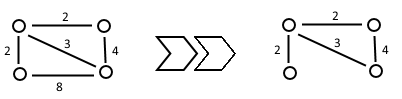
\includegraphics[scale=0.75]{Grafos/Grafo1}
\newline
\newline
\item 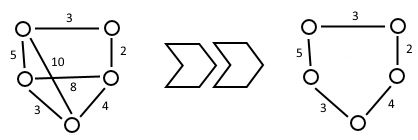
\includegraphics[scale=0.75]{Grafos/Grafo2}
\newline
\newline
\item 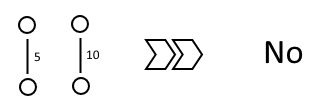
\includegraphics[scale=0.75]{Grafos/Grafo3}
\end{enumerate}

\newpage
\subsection{Desarrollo}

\noindent \textbf{\underline{Preliminares}}

Primero que todo, para poder resolver el problema, tenemos que abstraernos de lo que es una red y encontrar una estructura donde podamos almacenar los datos de una manera relevante para facilitarnos la resolución. La estructura elegida es un \textbf{\textit{grafo no dirigido}}, representado por una \textbf{\textit{matriz de adyacencia pesada}}. Si la matriz de adyacencia $A$ representa al grafo $G = (V,X)$, entonces la posición $A_{v1,v2} = A_{v1,v2} = x_{v1,v2} = x_{v1,v2}$, con $v1,v2 \in V$ y, $x_{v1,v2} \in X$ y es el peso de la arista que une a v1 y v2. En caso de que no exista arista que una ciertos 2 vértices ($p,q \in V$) del grafo, adoptamos que $A_{p,q} = (-1)$, como es el caso de $A_{p,p}$. Habiendo dicho esto, \textbf{\textit{cada vértice representa un equipo}} que sea parte de la red, y \textbf{\textit{las aristas reemplazan al costo de mantener una conexión entre 2 equipos}}.

\noindent \textbf{\underline{Idea}}

Volviendo a la resolución del trabajo, teniendo un grafo podemos aprovechar las útiles propiedades que posee, por ende de ahora en más no vamos a hablar más de red, servidor, equipos y costos sino de grafo, ciclo, vértices y peso de aristas respectivamente. Desde este punto de vista, el grafo que hay que armar es un \textbf{\textit{subgrafo generador}}, \textbf{\textit{conexo}} con \textbf{\textit{un sólo ciclo}} de \textbf{\textit{costo mínimo}}. Si uno quita la condición de que tenga al menos un ciclo, lo que nos queda es un grafo generador, conexo y sin ciclos de costo mínimo, en otras palabras un \textbf{\textit{árbol generador mínimo}}. Esto no resuelve el problema, pero está muy cerca ya que si obtenemos el AGM nos garantizamos un grafo sin ciclos de peso mínimo. Por ser un árbol, sabemos que con agregarle una arista pierde su propiedad árborea, ya que pasaría a tener exactamente un ciclo. Sin embargo, la elección de esa conexión a mantener no puede ser arbitraria para poder llevar a cabo nuestra tarea,  \textbf{\textit{debe ser una de las aristas de peso mínimo que no se encuentre colocada en el AGM que ya tenemos}}. Si no se elige la menos costosa, siempre se puede armar una red casi equivalente, pero que posea esa conexión más barata, para formar el servidor, que no es la que elejimos. Por ende, el resultado final consta de un grafo generador y conexo con un sólo ciclo que respeta la condición de costo total mínimo. En la sección de correctitud se demostrará como este proceso genera efectivamente una solución óptima.

\noindent \textbf{\underline{Ilustración}}

Para concretar la idea, lo que se realiza, en rasgos generales, es lo siguiente:

\begin{enumerate}
\item Toma de datos de la red para armar el grafo subyacente.
\item Si se puede armar el AGM en base a dicho grafo, se lo arma y se continúa al siguiente paso. Si no, indicamos que no es posible resolver la tarea.
\item Si hay al menos un enlace disponible que no haya sido utilizado en el paso 2), se busca y coloca la conexión de menor peso que no esté presente en el AGM obtenido en el paso 2).
\end{enumerate}

Para ilustrar el proceso:

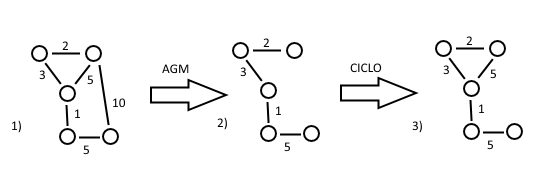
\includegraphics[scale=0.75]{Grafos/Proceso}

\noindent \textbf{\underline{Algoritmos usados y detalles importantes}}

Dentro de los algoritmos usados para la resolución, hay 2 de importancia: el algoritmo de prim, arma un AGM posible para un grafo input; una versión modificada al algoritmo de BFS que, dado un AGM y 2 nodos pertenecientes a él, devuelve la información del camino entre ambos para obtener los equipos pertenecientes al ciclo. Esto se requiere para dar formato correcto al output. Tanto los pseudo-códigos de ambos como de las sub-rutinas utilizadas se encuentran en la sección de complejidad para facilitar el análisis de ella.

\newpage
\subsection{Correctitud}

\noindent\textbf{\underline{Objetivo}}

Lo que queremos demostrar es que una manera de encontrar \textbf{\textit{una solución óptima}} es \textbf{\textit{construyendo un AGM subyacente}} y luego \textbf{\textit{colocarle la arista más liviana de las quue no fueron colocadas en el AGM}}, efectivamente formando un ciclo.

\noindent\textbf{\underline{Características de una solución óptima}}

Sabemos que una solución, tal vez no óptima, debe tener forma de \textbf{\textit{sub-grafo generador con uno o más ciclos}}. Llamando a la red $G$, supongamos que llamamos a la solución $S$. \textbf{\textit{Llamamos \boldmath$S_{i}$ a sub-grafo de $S$ tal que le quitamos i aristas que forman ciclos}}, de tal forma que $S_{i}$ sigue siendo conexo, donde 0 $\leq$ i $\leq$ (cantidad de aristas que forman ciclos en S). Para simplificar las cosas, $k =$ (cantidad de aristas que forman ciclos en S) $= m - (n-1)$. Necesariamente $m > (n-1)$ debido a que un sub-grafo generador debe tener al menos $(n-1)$ aristas y además tiene 1 o más ciclos. Como estamos quitando conexiones, sabemos que $p(S_{0})\leq p(S_{1}) \leq ... \leq p(S_{k})$, donde la función $p(R)$ nos indica el peso total para un grafo cualquiera $R$. En otras palabras, la solución es igual o mejor si tiene menor cantidad de ciclos. La razón por la cuál la relación de desigualdades no es estricta, es porque puede haber aristas de costo $0$ que formen ciclos, y si las quitamos no altera el costo del grafo. A cualquier solución se le puede hacer esta reducción de aristas, ya que sabemos que tienen 1 o más ciclos, de forma tal que abarcamos todo el espectro de soluciones. La solución minimal que podríamos armar en cada caso es un $S_{k-1}$. \textbf{\textit{Lo que queremos probar es que para toda solución \boldmath$S$, con \boldmath$S_{k-1} = H$, se cumple que, dada nuestra solución propuesta \boldmath$T$, \boldmath$p(T) \leq p(H)$}}. En términos menos formales, que la resolución planteada genera una red óptima.

\noindent\textbf{\underline{Demostración}}

Supongamos que no es cierta la relación anterior:\textbf{\textit{ existe alguna solución \boldmath$S$ tal que su \boldmath$H$, que es el resultado de sacar \boldmath$k-1$ aristas que forman ciclos de \boldmath$S$, tal que \boldmath$p(T) > p(H)$}}. Queremos llegar a algo absurdo que pruebe que lo postulado es es incorrecto, probando que lo contrario es cierto.
Tomamos $e$, la arista de mayor peso en el ciclo de $T$ con $T' = T - e'$, además $T'$ es AGM ya que le quitamos a nuestra solución la única arista que formaba ciclos, lo que nos queda es el AGM armado. Teniendo en cuenta esto, separamos en 2 casos:
\begin{enumerate}
\item[I.] El ciclo de $T$ y el ciclo de $H$ tienen alguna arista en común.
\item[II.] Sus ciclos no tienen aristas en común.
\end{enumerate}

\underline{Caso I:} Tomamos $e'$ de H, una de las que tienen en común. Tenemos que $H' = H - e'$ que es un Àrbol Generador. Sabemos que $p(e) \leq p(e')$, sino tomaríamos $T* = T' - e + e'$ que sería un árbol generador con menor peso que $T'$, pero $T'$ es AGM y eso es absurdo. Por ende, $p(e) + p(T) \leq p(e') + p(H') \iff p(T) \leq p(H)$, pero habíamos asumido lo contrario. Llegamos a un absurdo.  \newline
\indent \underline{Caso II:} Tomamos $e*$ cualquier arista del ciclo de H y la quito, entonces tengo $H* = H - e*$. De nuevo, $H*$ es un árbol generador entonces $p(T') \leq p(H*) \iff p(T') + p(e) \leq p(H*) + p(e*) \iff p(T) \leq p(H)$, pero habíamos asumido lo contrario. Llegamos a un absurdo.

Como son 2 casos disjuntos y nuestra solución S es genérica, probamos que es cierto para todo caso. Con lo cuál probamos lo que habíamos postulado.

\noindent\textbf{\underline{Comentarios Adicionales}}

\begin{itemize}
\item Somos conscientes que a la demostración le falta formalidad. Estuvimos ajustados de tiempo ya que no se nos ocurriá como hacerla.
\item La función p está sobrecargada, se ajusta a lo que le pases como parámetro devolviendo el peso total de un grafo o de una arista dependiendo el caso.
\end{itemize}

\newpage
\subsection{Complejidad}

\noindent \textbf{\underline{Aclaraciones pertinentes}}

\begin{enumerate}
\item Algunas definiciones de tipo: peso es int, nodo es int, grafo es vector$<$vector$<$peso$>>$, pesoPredecesor es pair$<$peso,nodo$>$, vectorPesoPredecesor es vector$<$pesoPredecesor$>$, parNodo es pair$<$nodo,nodo$>$, tuplaSolución es pair$<$grafo, bool$>$, tuplaCiclo es pair$<$parNodo, bool$>$, predecesores es vector$<$nodo$>$, list$<$nodo$>$ es camino. Las estructuras utilizadas son las provistas por la STL y los tipos de datos involucrados son los estándares de C++.
\item Los componentes del pseudo-código que estén descriptos en palabras, son operaciones que tienen complejidad temporal O(1), excepto que se explicíte lo contrario en algún/os caso/s particular/es.
\item No se tendrán en cuenta los costos de entrada de datos (input) y salida (output). Cabe aclarar que, si bien el algoritmo de BFS se encuentra únicamente para dar formato pedido a la salida, este sí va a ser sometido a un análisis intrínseco debido a que lo realizado por el mismo no es trivial.
\item Ciertas subrutinas no van a ser plasmadas en pseudo-código ya que consideramos que son simples de entender (iterar una matriz, iterar una lista, etc) y puede haber un remplazo de su correspondiente pseudo-código con un párrafo o algunas frases que expliquen lo que harían de manera que esté claro lo que llevan a cabo. De la misma forma se va a mencionar su costo temporal.
\end{enumerate}

\noindent \textbf{\underline{Pseudo-códigos y cotas de complejidad}}

Comenzando por el algoritmo de prim, el siguiente es su pseudo-código:

\begin{lstlisting}
tuplaSolucion prim(grafo& input, int& costoTotal)

int n = input.size()

grafo res(n,n)
vectorPesoPredecesor diccionario(n)

//Indica, para cada nodo, si fue agregado al AGM
vector<bool> unidos(n)
unidos[0] = true

//Variables principales
int cn = 0
nodo nodoActual = 0
bool sigo = true

//Variables Auxiliares
pesoPredecesor conexionMinFueraAGM;
nodo nodoAConectar;

mientras (cn < n && sigo)
	para todo nodo i desde 0 hasta n-1
		si (i no esta conectado) && input[nodoActual,j]} >= 0 &&
		    input[nodoActual,i] < diccionario[i].peso)
		    
			diccionario[i] = <input[i,j],nodoActual>
		fin si
	fin para

	conexionMinFueraAGM = diccionario[0]
	nodoAConectar = 0

	//Recorro las aristas almacenadas en diccionario y tomo la menos pesada 		que conecte un nodo que ya este en el AGM con otro que no



	para todo nodo i desde 0 hasta n-1
		si (i no esta conectado) && (diccionario[i].peso >= 0)
			si diccionario[i].peso < conexionMinFueraAGM.peso
				conexionMinFueraAGM = diccionario[i]
				nodoAConectar = i
			fin si
		fin si
	fin para
	Si (hay encontre alguna arista para unir)
		unir(res,nodoAConectar, conexionMinFueraAGM.nodo,conexionMinFueraAGM.peso)
		unidos[nodoAConectar] = true
		nodoActual = nodoAConectar
		costoTotal += conexionMinFueraAGM.peso
		cn++
	Si no
		sigo = false
		cn++
	fin si
fin mientras

return <res, (sigo) || (cn == n))>
fin
\end{lstlisting}


\begin{itemize}
\item Crear el grafo res toma $\Theta(n^2)$. Las declaraciones de 'diccionario' y 'unidos' cuesta $\Theta(n)$.
\item El while (lineas 22 - 58) itera $n$ veces, por ende su costo esta caracterizado por $n*O(cuerpoWhile)$. No es $\Theta$ ya que si no hay un AGM subyacente al grafo 'input', la rutina no repite el cuerpoWhile tantas veces como nodos haya.
\item El for (lineas 24 - 30) realiza $n$ iteraciones de complejidad $O(1)$, por ende su costo total es $O(n)$.
\item El for (lineas 38 - 45) realiza $n$ iteraciones con costo temporal $O(1)$. Su costo total es $O(n)$.
\item Como el resto de las operaciones tienen costo temporal constante, se ve que el costo del cuerpoWhile $= O(2n) = O(n)$. Entonces, el while mencionado anteriormente es $O(n^2)$, por propiedades de la función $O$.
\item Se devuelve el grafo 'res' por copia y un booleano, dejando un costo de $\Theta(n^2)$ debido al tamaño de la matriz.
\end{itemize}

Finalmente, si $f(n)$ es la función que describle la complejidad del algoritmo de prim propuesto, sabemos que $f(n) \in 2\Theta(n^2) + \Theta(n) +  O(n^2)$. Utilizando propiedades de las funciones de orden y que si $g(n) \in \Theta(h(n)) \Rightarrow g(n) \in O(h(n))$, obtenemos que $f(n) \in O(n^2)$.

Una vez obtenido el AGM, debemos encontrar la arista menos costosa que pertenezca a la red que no se encuentre en el AGM:

\begin{lstlisting}
tuplaCiclo encontrarConexionMinParaAnillo(grafo& input, grafo& AGMInput)

int n = AGMInput.size()
parNodo conexionCostoMin = <0,0>
bool existe = false;

para todo nodo i desde 1 hasta n-1
	para todo nodo j desde 0 hasta i
		si (hay arista entre i,j en input pero no en AGM)
			si (input[i][j] < input[conexionCostoMin.nodo1][conexionCostoMin.nodo2])
			conexionCostoMin = <i,j>
			existe = true
			fin si
		fin si
	fin para
fin para
return <conexionCostoMin, existe>
fin
\end{lstlisting}

Si llamamos $g(n)$ a la función que indica el orden de complejidad de dicho algoritmo, podemos decir que: 
$g(n) \in \Theta(\sum\limits_{i=1}^{n/2} i) = \Theta(\dfrac{(n/2)*((n/2) - 1))}{2}) = \Theta((n^2/2) - n) = \Theta(n^2)$. 

\noindent En particular, por propiedad de la función $\Theta$, $g(n) \in O(n^2)$.


Resta ver el pseudo-código del BFS Modificado y dar su función de complejidad:

\begin{lstlisting}
predecesores BFSMod(grafo& AGM, nodo& inicio, nodo& destino)

int n = AGM.size()
predecesores predecesores(n)
vector<bool> visitados(n)
cola<nodo> noVisitados

visitados[inicio] = true
noVisitados.push(inicio)

nodoActual = inicio

mientras (noVisitados no este vacia) && (nodoActual != destino)
	noVisitados.pop()
	
	para todo nodo i desde 0 hasta n-1
		si (i no fue visitado) && (hay arista entre nodoActual e i en AGM)
			predecesores[i] = nodoActual
			visitados[i] = true
			cola.push(i)
		fin si
	fin para
	
	nodoActual = cola.front()
fin mientras

return predecesores
fin
\end{lstlisting}

\begin{itemize}
\item Las declaraciones de los vectores (lineas 4-5) toman $O(n)$, por otra parte la creación de la cola vacia se realiza en tiempo $O(1)$.
\item El while (lineas 13-25) itera tantas veces como nodos visite entre el inicio y el destino, su peor caso es que atraviese todos los nodos antes de lograrlo, lo cuál nos deja con una complejidad de $n*O(cuerpoWhile)$.
\item El for (lineas 16-22) realiza n pasos donde se ejecutan operaciones con costo $O(1)$, la complejidad resultante de él resulta $O(n)$.
\item Dado los 2 ítems anteriores, concluimos que la complejidad del while es $O(n^2)$.
\item El vector predecesores se devuelve por copia, temporalmente eso requiere $O(n)$ tiempo.
\end{itemize}

Llamaremos $h(n)$ a la función que caracteriza la complejidad de este algoritmo. Por todo lo mencionado, $h(n) \in O(n^2) + 3O(n)$, lo que implica, por propiedades de la función de orden O, que $h(n) \in O(n^2)$.

\noindent \textbf{\underline{Conclusión}}

La resolución del problema, sin tener en cuenta el input y el output, utiliza 1 llamado de cada uno de los algoritmos mencionados. Denominaremos $c(n)$ al costo de resolver el problema $\Rightarrow c(n) \in f(n) + g(n) + h(n) \Rightarrow c(n) \in O(n^2) + O(n^2) + O(n^2) = 3O(n^2) = O(n^2)$
Finalmente, la complejidad de la solución planteada es estrictamente mejor que $O(n^3)$, con lo cuál se cumple lo pedido por la empresa.

\newpage
\subsection{Experimentación}

\noindent \textbf{\underline{Introducción}}

Para la experimentación, se midieron 2 casos: promedio, peor y aumentando la cantidad de equipos sin aumentar la cantidad de aristas. Estos 3 escenarios lograron mostrar que se cumplió con la cota de complejidad temporal pedida y nos dieron ciertas conclusiones interesantes.
La técnica utilizada para tomar valores fue la siguiente: construimos generadores para cada caso particular, ellos nos generaron 100 instancias distintas de cada uno de sus casos, luego se llevaban acabo 100 repeticiones de resolución sobre cada instancia. Sobre cada instancia particular, tomabamos su mejor tiempo, debido a que es el valor que mejor representa el tiempo actual que tomó resolver el ejercicio. Es sabido que el cpu atiende muchas tareas en simuláneo y por ende es complicado medir efectivamente el tiempo real de la rutina ya que deberíamos hacer que el procesador sólo ejecute la rutina frenando toda otra actividad del equipo. Habiendo hecho esto, tomamos el promedio de las mediciones de cada instancia, lo que nos da una buena aproximación. Las mediciones están hechas en segundos y el tamaño está medido en $n$, la cantidad de equipos. Para cada caso particular se detallará cuál es la relación entre el n y la cantidad de conexiones para poder hacer un análisis más minucioso.

\noindent \textbf{\underline{Gráficos y conclusiones}}

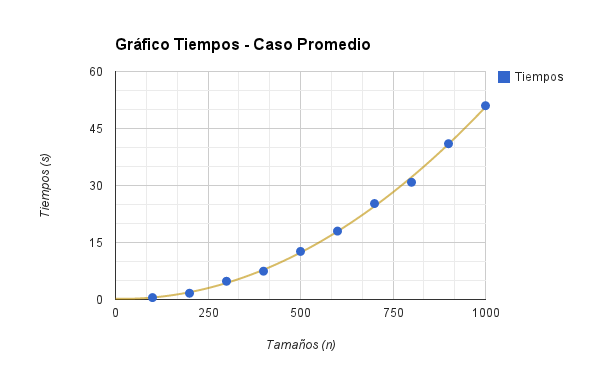
\includegraphics[scale=0.60]{Grafos/Grafico_Caso_Promedio}

Un caso sin sorpresas. Ayuda a ver cierta curvatura polinómica que evidencia la complejidad temporal. Se puede notar, para ciertos tamaños de instancias, que el incremento no es regular. Esto sucede porque pueden haber casos que se descartan tempranamente ya que esos grafos no poseen un AGM subyacente. Para estos casos, la cantidad de aristas, m, esta acotada de la siguiente manera $0 \leq m \leq \frac{n*(n-1)}{2}$. En estas situaciones puede suceder que el factor que mas aporta a los tiempos de ejecución varíe entre la cantidad de equipos y la cantidad de aristas. Más adelante, basandonos en otras circumstancias, veremos que es lo que más determinante.

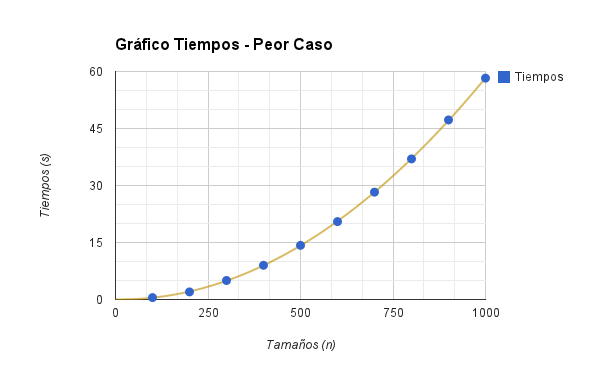
\includegraphics[scale=0.60]{Grafos/Grafico_Peor_Caso}

Se puede observar que la cota de complejidad es efectivamente polinomial. La cantidad de conexiones, dadas estas circumstancias, están fijas y equivalen a $\frac{n*(n-1)}{2}$, formando un grafo completo. La diferencia entre casos peores y promedios es notable, llegando a tener diferencias de más de 6 segundos para ciertas instancias. En estos casos, el predominio está claramente dado por el número de conexiones en materia de tiempos. El crecimiento es mucho más regular debido a que no se puede dar un caso de rápida terminación, un grafo completo siempre contiene un AGM.

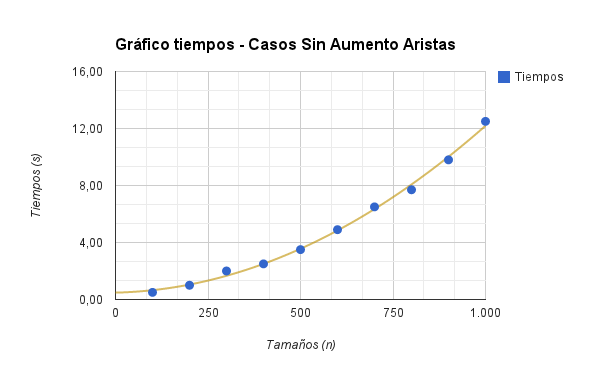
\includegraphics[scale=0.60]{Grafos/Grafico_Caso_Sin_Aumento_Arista}

Lo que se hizo en este caso es tomar un grafo de 100 nodos que sea completo, medir los tiempos, e ir aumentando en 100 la cantidad de nodos sin generar nuevos ejes, de forma tal que los grafos son inexorablemente inválidos para presentar una solución ya que cada nodo nuevo aporta una componente conexa adicional. ¿Qué es lo que genera el aumento de tiempos? El tamaño de la matriz de adyacencia pesada. Que no haya conexiones adicionales, no implica que pueda optar por no recorrer toda la matriz en pos de armar el AGM. Si bien esta caso termina siempre en el nodo 101, para todos los nodos anteriores debe iterar hasta n en busca de nuevas conexiones. Esto nos da la pauta de que, para esta problemática en particular, la elección de una estructura alternativa que favorezca no iterar de más, como lista de adyacencias pesadas, hubiese sido una mejor decisión. No por la cota de complejidad, sino por los tiempos en la práctica.

\noindent \textbf{\underline{Comentarios finales}}

\begin{enumerate}
\item Nos hubiese gustado, en los 2 primeros gráficos, comparar contra funciones cuadráticas. No llegamos a hacerlo por cuestiones de tiempo y limitaciones del software elegido.
\item La idea de cambiar de estructura a listas de adyacencia se nos ocurrió pasado el tiempo de haber armado la rutina entera, los pseudo-códigos y gran parte del informe, incluyendo la complejidad. Una buena lección para recordarnos que el trade-off del acceso a una posición en $O(1)$ puede costar significativamente.
\end{enumerate}